\section{Wybór danych i modelu}

\subsection{Model}
Jako podstawę naszego modelu wybraliśmy musicNN (\url{https://github.com/jordipons/musicnn}), publicznie dostępny model splotowy. Wyjściem modelu jest uporządkowanie 50 cech, obejmujących styl oraz instrumenty.

Tagi: guitar, classical, slow, techno, strings, drums, electronic, rock, fast, piano, ambient, beat, violin, vocal, synth, female, indian, opera, male, singing, vocals, no vocals, harpsichord, loud, quiet, flute, woman, male vocal, no vocal, pop, soft, sitar, solo, man, classic, choir, voice, new age, dance, male voice, female vocal, beats, harp, cello, no voice, weird, country, metal, female voice, choral.

Wyjściem z modelu są cechy ważne w określaniu gatunku, ale inne gatunki niż te określane przez nasz model. Dodatkowo jego rozmiar jest mały, co pasuje dla naszego docelowego zastosowania, oraz potrzeby wielokrotnego treningu z różnymi nastawami. W związku z tym model został punktem wyjścia do optymalizacji.


Wagi, na podstawie których chcemy transferować wiedzę, były wytrenowane na zbiorach MagnaTagATune. W repozytorium dostępne są również wagi wynikające z ćwiczenia na Million Song Dataset, z odpowiednimi tagami.



Ponieważ model powienien przyjmować dane o różnej długości, wejściowe nagrania dzielone jest na 3-sekundowe segmenty, z których tworzone są melspektrogramy o rozmiarach 187x96. Na wejście modelu podawany jest logarytm z ich wartości (rys. \ref{fig:musicnn}). Wyjścia o rozmiarze 1x50 można zagregować dla całego utworu i uśrednić.


\begin{figure}[ht]
    \centering
    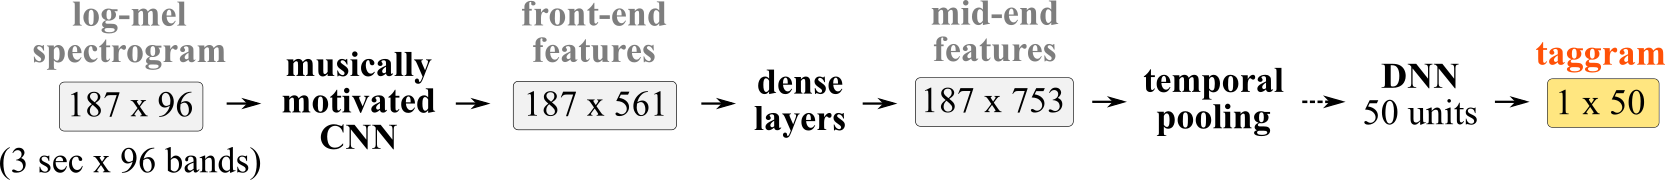
\includegraphics[width=\linewidth]{img/musicnn.png}
    \caption{Struktura modelu musicnn}
    \label{fig:musicnn}
\end{figure}



Przy trenowaniu modelu na dostępnym sprzęcie, uzyskana została nastepująca charakterystyka:
\begin{table}[h]

    \centering

    \begin{tabular}{|l|c|}
        \hline
        \textbf{Parametr}               & \textbf{Wartość} \\
        \hline
        Liczba parametrów               & 785245           \\
        Czas wnioskowania               & TODO             \\
        Czas treningu pojedynczej epoki & TODO             \\
        Wymagania pamięciowe            & TODO             \\

        \hline
    \end{tabular}

    \caption{Porównanie modeli}
    \label{tab:modele}

\end{table}


\subsection{Zbiór danych}
Do wytrenowania wykorzystany został zbiór FMA (Free Music Archive) \url{https://github.com/mdeff/fma/tree/master} \cite{fma_dataset}

Posiada on kilka podzbiorów, oraz hierarchiczną strukturę gatunkową, co pozwoliło nam na pobranie najmniejszej wersji zbioru i przetestowanie modelu przed podjęciem decyzji o ostatecznych wielkościach zbiorów. Zbiór zgadza się z założeniami projektowymi, zawiera nagrania mp3, a był wykorzystywany (według autorów) w ponad 100 artykułach naukowych.


Inny zbiory danych wykorzystywane w muzyce to chociażby GTZAN, MagnaTagATune, Million Song Dataset, przedstawione w tabeli \ref{tab:datasets}.

\begin{table}[h]
    \centering
    \begin{tabular}{|p{3cm}|p{3cm}|p{2.7cm}|p{6cm}|}
        \hline
        \textbf{Zbiór}                                        & \textbf{Liczba klas}         & \textbf{Liczba \ nagrań} & \textbf{Uwagi}                                                                                                                                       \\
        \hline
        FMA-small                                             & 8 gatunków (hierarchicznych) & 8000 (30s)               & Dla FMA gatunki są ustawione w hierarchię drzewiastą, od najbardziej ogólnych do szczególnych. Tutaj najbardziej ogólne gatunki. Zbiór zrównoważony. \\
        \hline
        FMA-medium                                            & 16 gatunków                  & 25000 (30s)              & Gatunki najbardziej ogólne. Zbiór niezrównoważony.                                                                                                   \\
        \hline
        FMA-large                                             & 161 gatunków                 & 106574 (30s)             & Zbiór niezrównoważony.                                                                                                                               \\
        \hline
        FMA-full                                              & 161 gatunków                 & 106574                   & Nieprzycięte nagrania. Zbiór niezrównoważony                                                                                                         \\
        \hline

        GTZAN \cite{tzanetakis2002}                           & 10 gatunków                  & 1000 (30s)               & 30-sekundowe nagrania                                                                                                                                \\
        \hline
        MagnaTagATune\cite{magnatagatune_dataset}             & 188 tagów                    & 25877 segmentów (30s)    & Do ewaluacji często używane 50 najczęstszych tagów \cite{ferraro2020}.
        \\
        \hline
        Million Song Dataset (MSD)\cite{million_song_dataset} & $>$ 2000 tagów               & 1000000                  & Nie ma dostępnych nagrań, tylko cechy utwórów. Do ewaluacji często używane 50 najczęstszych tagów \cite{ferraro2020}.                                \\
        \hline
    \end{tabular}
    \caption{Porównanie muzycznych zbiorów danych}
    \label{tab:datasets}
\end{table}